First, the indentation into an elastic sphere tests and validates our FEM approach. Indentation of the AFM tip into the soft spherical sample, with elastic modulus $E = 1000$kPa, exerts a compressive force $\mathbf{F}$ onto the sample. Illustrated in Figure \ref{fig: Capped-Sphere-Plot}A, the compression of the sphere enhances the perceived indentation depth, $\delta_{12}$, and indentation force is distributed between the reaction at the base and the indenter such that the perceived force, $F_{12}$, is diminished. 

%This necessitates accounting for the indentation between the indenter and the surface and the indentation between the surface and the base. The forces and displacement across the AFM tip surface are mapped to a central reference point within ABAQUS. 

Figure \ref{fig: Capped-Sphere-Plot}B shows the extracted force-indentation data for various surface-indenter ratios $\frac{r}{R}$ scaled in dimensionless units. The simulations show the characteristic indentation force curve. Increasing the surface radius ($R$) decreases the bounded area, indicating heightened energy requirements for compressing smaller spheres. These more complex compression dynamics are expected to deviate from the theoretical models, which model linear elastic responses\cite{kontomaris2019determination}. The compression necessitates the Double Contact model, which more accurately models AFM indentations. 

%However, we expect the AFM tip to produce a curve with transitional behaviour around $\delta/R=0.65$ as the indenter moves from the spherical portion to the conical.
%Moreover, the finite extent of elastic spheres, especially at large tip-surface ratios, deviates from the Hertz and Sneddon models, which describe elastic half-spaces with infinite extent in all directions\cite{kontomaris2019harmonic}. 

The dimensionless force, $\frac{F}{E^*R^2}$, as it varies with relative indentation depth, $\frac{r}{R}$, is fitted to the theoretical models as shown in Figure \ref{fig: Capped-Sphere-Plot}C. The Double Contact and Hertz model produced qualitatively tight fits. In contrast, the Sneddon model displays more pronounced curvature, overestimating the deformation from the spherical AFM tip compared to a sharper conical tip. Moreover, model accuracy across various surface radii ($r$) can be assessed by comparing the measured Young's modulus ($E_{AFM}$), extracted as a fitting parameter\cite{sun2021determination, DIMITRIADIS20022798, kontomaris2019determination}, with the true Young's modulus of the sample. 

The Hertzian model underestimates Young's modulus, shown in Figure \ref{fig: Capped-Sphere-Plot}D, underfitting by approximately half across surface range.  This reduction is consistent with the decrease in indenter reaction force experienced when compressing the sample. The Sneddon model shows a poor fit, converges to zero, indicating the spherical indentation is dominant which is consistent with the relative size of the spherical termination. 

%This highlights the importance of the contribution of compression at the base of the sample. 

\begin{figure}[htp]
    \centering
    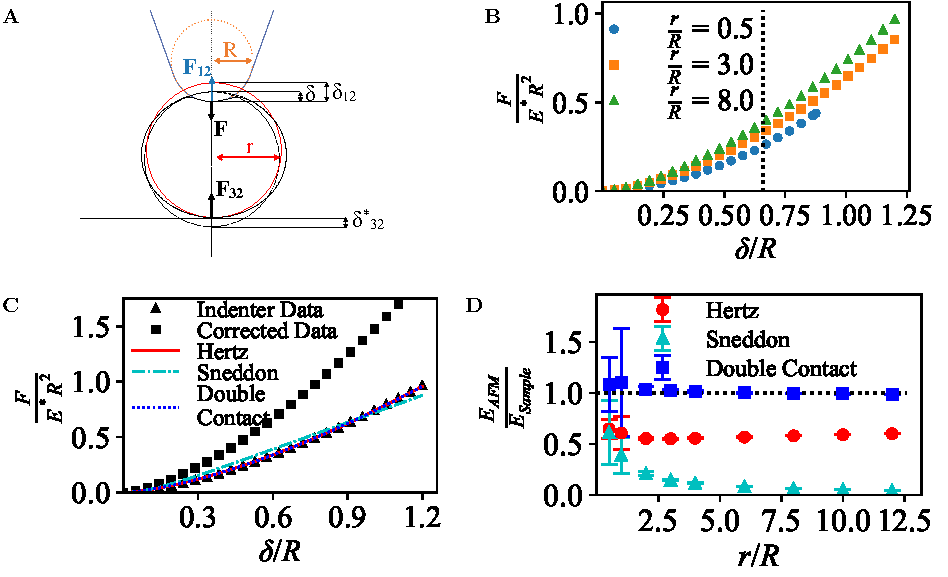
\includegraphics[width=1\linewidth]{Figures/Figure2.pdf}
    \caption{\label{fig: Capped-Sphere-Plot} (A) Illustration of double contact experienced by spherical sample. For indentation $\delta$, indenter displacement $\delta_{12}$, surface compression $\delta^*_{32}$, indentation force $F$, indenter reaction force $F_{12}$, and base reaction force $F_{32}$. Corrected values for the indentation depth, $\delta$, are calculated by subtracting the surface compression at its base, $\delta^*_{32}$, from the indenter's displacement $\delta_{12}$. (B) Force curve for indentation $\delta/R$ into the elastic sphere of varying radius, r/R. (C) Plot of fitted contact models over  dimensionless force, $\frac{F}{E^*R^2}$, against relative indentation, $\frac{\delta}{r}$ range. For surface-indenter ratios, $r/R = 3.0$. (D) Variation of relative Young's Modulus, $\frac{E_{AFM}}{E_{Sample}}$ for varying surface-indenter ratios, $r/R$.}
\end{figure}

In comparison, the Double Contact models converge to the expected Young's modulus within the confidence interval. At small surface radii, the AFM tip is comparable size to the surface. Force are distributed over substantial portion of the surface producing excessive compression and shear forces. Consequently, this causes significant errors and deviation from the theoretical models along with the contradiction of the assumption of infinite surface extent. The error decreases as surface radius increases and compressive effects lessen although a minor offset is expected due to the indenters conical portion. Overall, these results further validated our ABAQUS modelling.

%Fitting data with a restricted indentation depth, excluding the conical section at depths greater than $\delta/R=0.65$, the force curves highlight the transitional behaviour. As shown by the dashed line in Figure \ref{fig: Capped-Sphere-Plot}, the Double Contact model produces tighter fits at small indenter-surface ratios when considering indentations with only the spherical portion. 